\chapter{Implementation}

In this chapter, we will go through our \emph{application generator}, explaining in detail how it works and how it is implemented from the inside. We will focus both on the \emph{platform} aspect and the \emph{framework} aspect. As for the \emph{platform} aspect, we will show how a non-developer can use the new \emph{platform} to generate and share Linked Data based applications. As for the \emph{framework} aspect, we will provide a potential developer with a step-by-step guide for how to implement a new \emph{visualizer}. As our generator is built on top of LinkedPipes Visualization, its official name is LinkedPipes Application Generator. For brevity, we will refer to it simply as to (our) \emph{application generator}. 

\section{Overview}

Before we dive into technical details, let us walk the reader through the \emph{application generator} from a user perspective. We will start by describing a sample use case scenario.

\subsection{Sample use case}

In this scenario, we will utilize the D3.js Chord Visualizer and the Asylum Seekers 2015 data set. Both will be properly described later in a separate chapter dedicated to this particular visualizer.


\begin{figure}
	\centering
	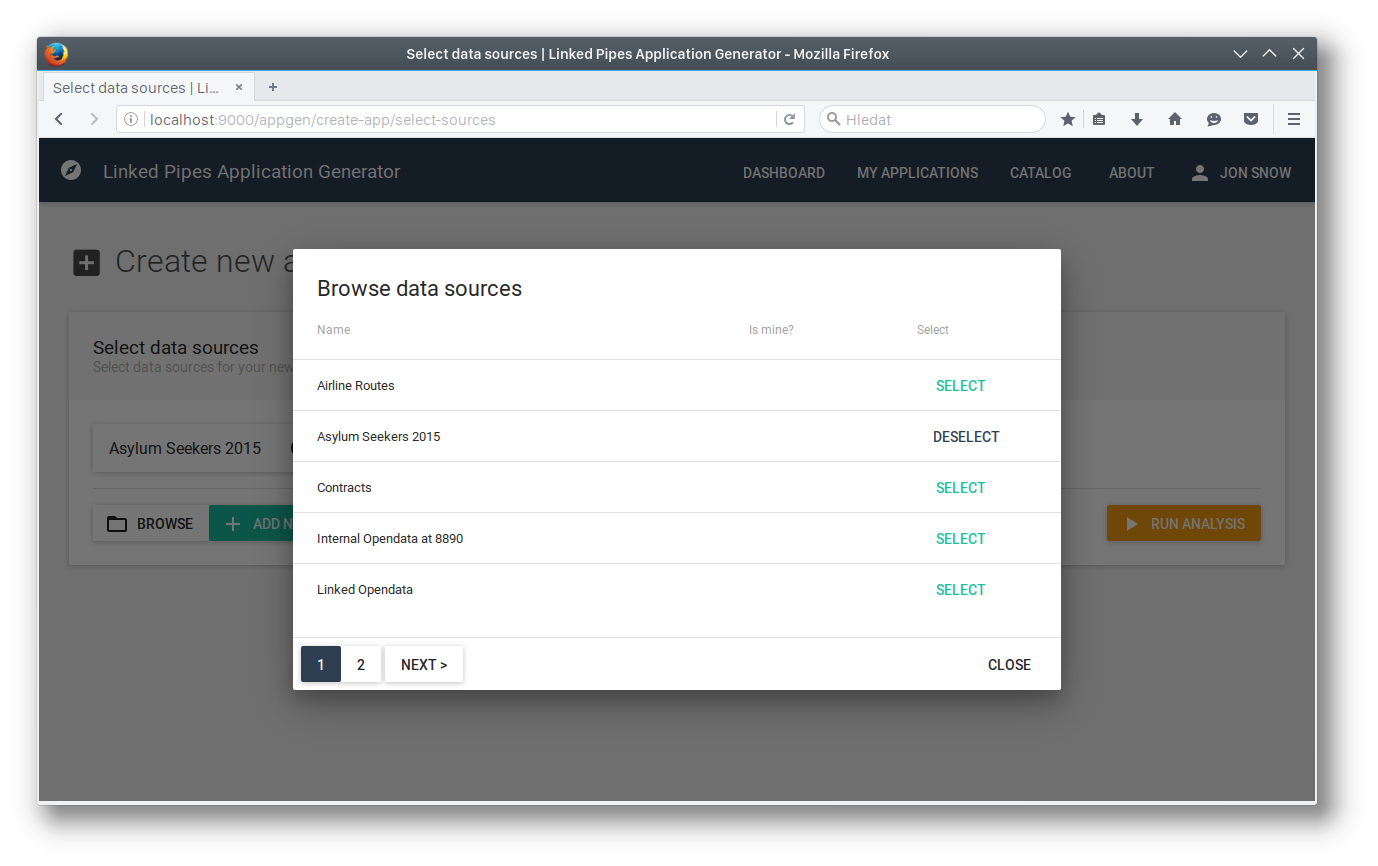
\includegraphics[width=145mm]{img/05_scenario_01_browse_data_sources.png}
	\caption{Citadel on the Move: A sample generated application. Source of picture \cite{citadel_agt_doc}}
	\label{fig:scenario-01-browse-data-sources}
\end{figure}

\begin{figure}
	\centering
	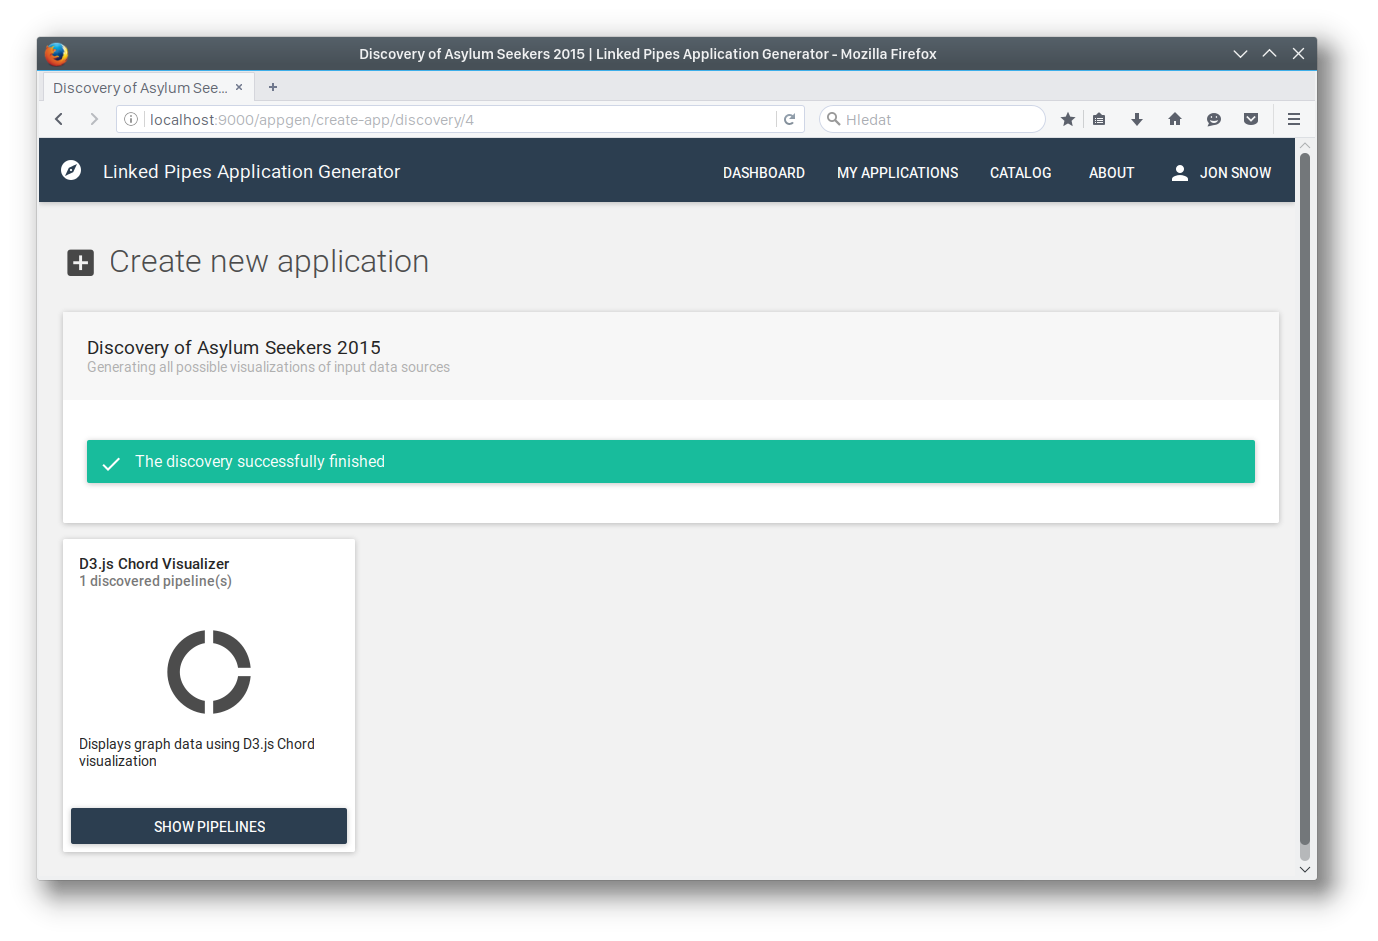
\includegraphics[width=145mm]{img/05_scenario_02_discovery_result.png}
	\caption{Citadel on the Move: A sample generated application. Source of picture \cite{citadel_agt_doc}}
	\label{fig:scenario-02-discovery-result}
\end{figure}

\begin{figure}
	\centering
	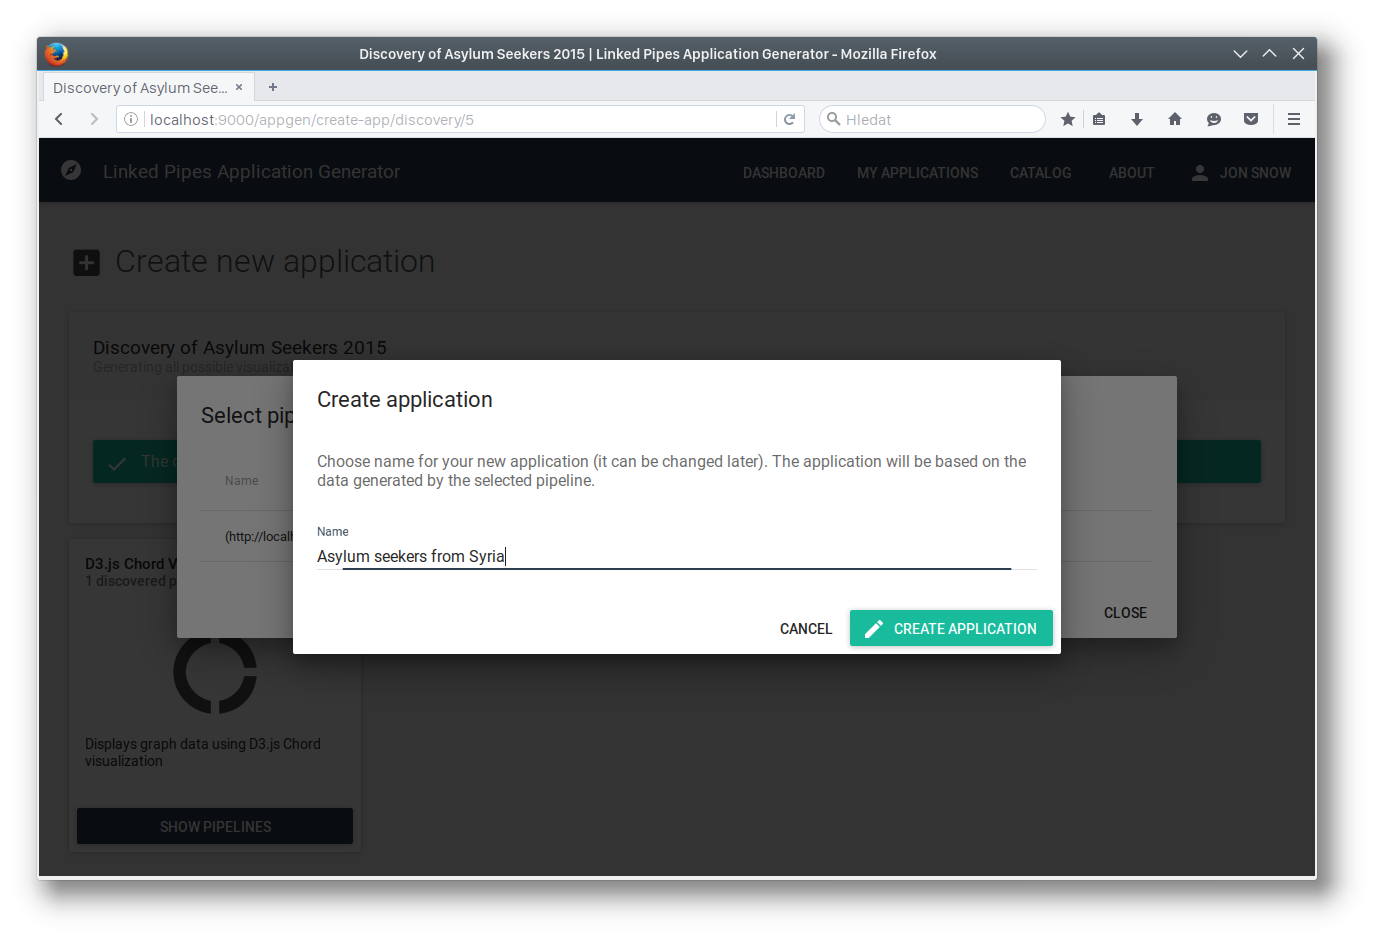
\includegraphics[width=145mm]{img/05_scenario_03_create_application.png}
	\caption{Citadel on the Move: A sample generated application. Source of picture \cite{citadel_agt_doc}}
	\label{fig:scenario-03-create-application}
\end{figure}


\subsection{User agenda}

\subsection{Managing data sources}

\subsection{Pipeline discovery}

\subsection{Configuring application}

\subsection{Publishing application}

\subsection{Miscellaneous}



\section{Inner architecture}

% Alternative frontend

% Platform vs 



\section{Scala Backend}

% Simple, following the architecture of LinkedPipes Visualization

% Two entry endpoints URLs: platform and application

% Each visualizer has its own controller

% Cache?


\section{Frontend development stack}

\subsection{ES6 and Babel compiler}

\subsection{React}

\subsection{Redux}

\subsection{Reslect}

\subsection{React-router}



\section{Frontend framework architecture (???)}

\subsection{Ducks}

\subsection{Modules}



\section{Integrating a new visualizer}

\subsection{LDVM component}

\subsection{Frontend module}

\subsection{Configurator interface}

\subsection{Application interface}

\subsection{Backend}

\subsection{Fetch and display sample RDF data}



\section{Advanced framework features}

\subsection{Saving and loading application configuration}

\subsection{Multiple language support}

\subsection{Label dereferencing}

\subsection{Custom label editor}

\subsection{Embedding applications}

\subsection{Miscellaneous}
